\documentclass[tikz,border=8pt]{standalone}
\usepackage{lmodern}
\usetikzlibrary{arrows.meta,positioning}
\begin{document}
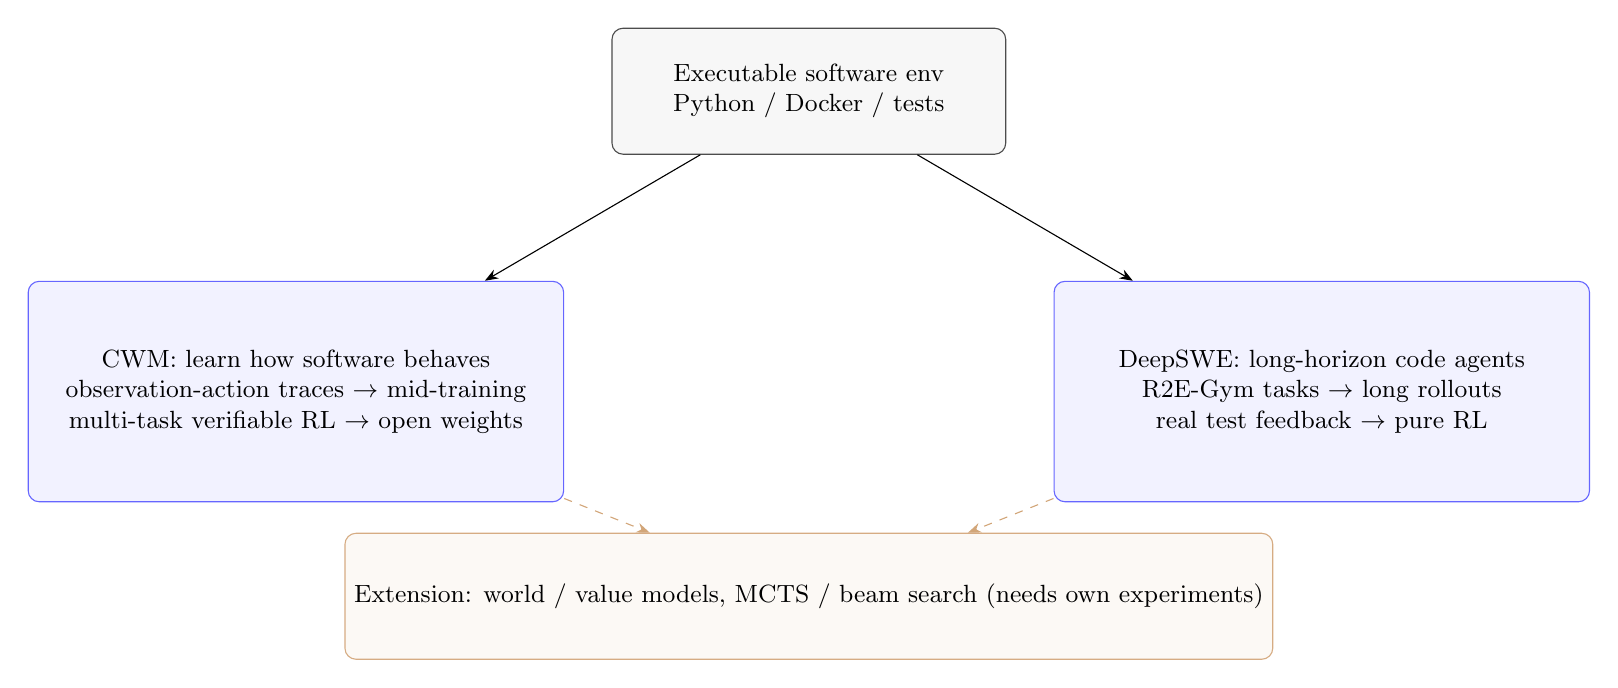
\begin{tikzpicture}[>=Stealth,every node/.style={align=center,font=\small},box/.style={rounded corners,draw=black!70,fill=black!3,minimum height=16mm},main/.style={box,draw=blue!60,fill=blue!5,minimum width=68mm,minimum height=28mm}]
\node[box,minimum width=50mm] (env) {Executable software env\\Python / Docker / tests};
\node[main,below left=16mm and 6mm of env] (cwm) {CWM: learn how software behaves\\observation-action traces $\to$ mid-training\\multi-task verifiable RL $\to$ open weights};
\node[main,below right=16mm and 6mm of env] (deep) {DeepSWE: long-horizon code agents\\R2E-Gym tasks $\to$ long rollouts\\real test feedback $\to$ pure RL};
\node[box,draw=brown!65,fill=brown!5,below=14mm of env,yshift=-34mm,minimum width=105mm] (ext) {Extension: world / value models, MCTS / beam search (needs own experiments)};
\draw[->] (env)--(cwm); \draw[->] (env)--(deep); \draw[->,dashed,brown!70] (cwm)--(ext); \draw[->,dashed,brown!70] (deep)--(ext);
\end{tikzpicture}
\end{document}
